\newcommand{\nl}{$n_{\ell}$ }
\newcommand{\km}{\textless k \textgreater}
\chapter{Structure des réseaux sans-échelle non corrélés: couches et plus court chemin}
\label{sec3}
L'objectif principal de ce chapitre vise à prédire quel sera le comportement des systèmes en réseau sur la base des propriétés structurelles mesurées et des règles locales régissant les sommets individuels. Comment, par exemple, la distribution des degrés du réseau affectera-t-elle sa  structure et ses propriétés ?

\section{Introduction}

De nombreux réseaux du monde réel qui ont été décrits précédemment, tels que le WWW et les réseaux de collaboration, grandissent avec le temps. Par conséquent, il est raisonnable de considérer les graphes de taille croissante et d'étudier la structure de ces réseaux ayant souvent la propriété sans-échelle (voir Section.\ref{s-libre-echelle}). 
La communauté scientifique, en s'appuyant sur des idées issues d'une grande variété de disciplines, a fait un excellent départ sur la caractérisation et la modélisation de la structure des réseaux, mais il n 'y pas encore des progressions théoriques cruciaux dans ce domaine \cite{Ne2003}. Ici nous allons envisager ces problèmes en donnant quelques contributions à ces études concernant la structure des réseaux sans-échelle. En effet, on a trouvé pour la première fois les expressions explicites des couches, ainsi que, des formules plus précises du plus court chemin par rapport aux anciens résultats existant dans la littérature. 
\section{Mesurer les lois de puissance}
Identifier un comportement de la loi de puissance dans les systèmes naturels ou artificiels peut être difficile.  La stratégie standard utilise le fait que la courbe d'une quantité avec une distribution de loi de puissance apparaît comme une ligne droite lorsqu'elle est tracée sur des échelles logarithmiques. Il suffit toutefois de faire une simple courbure et de la tracer sur des échelles logarithmiques pour voir s'elle semble droite ou non (voir Fig.~\ref{sans-echelle-3}).\\

\begin{figure}[h!]
	\centering
	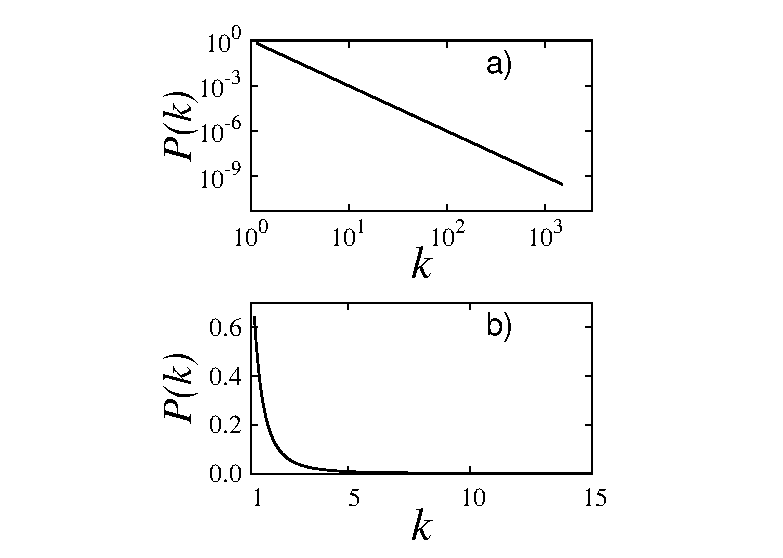
\includegraphics[scale=1.2]{./figures/fig-sans-echelle}
	\caption{Illustration de la loi de puissance pour une fonction, $P(k)=k^{-\gamma}$, avec l'exposant $\gamma=3$. Dans a) l'échelle est logarithmique et dans b) l'échelle est linière.}
	\label{sans-echelle-3}
\end{figure}
Pour révéler une loi de puissance, il vaut mieux, comme nous avons vu, tracer les courbure sur des échelles logarithmiques, et quand nous faisons cela pour nos données, nous voyons la forme linéaire caractéristique de la loi de puissance.
Cependant, la méthode n'est pas très bonne à certains égards. En particulier, l'extrémité de la droite de la distribution est bruyante en raison d'erreurs d'échantillonnage. Le fait que la distribution diminue dans l'extrémité, cela signifie que chaque valeur mesuré ne contient que quelques échantillons. Ainsi, les fluctuations dans les valeurs mesurées sont grandes et cela apparaît comme une courbe bruyante sur la figure. Une façon de traiter cela serait simplement de jeter les données dans la queue de la courbe. Mais il y a souvent des informations utiles dans ces données, car de nombreuses distributions suivent une loi de puissance seulement dans la queue.


Une solution alternative consiste à faire varier la largeur des cases dans notre courbe. Si nous allons faire cela, nous devons aussi normaliser les comptes d'échantillons par la largeur des valeurs mesurées. Autrement dit, le nombre d'échantillons dans un largeur $\Delta x$ devrait être divisé par $\Delta x$ pour obtenir un compte par intervalle unitaire de $x$. Ensuite, le nombre d'échantillons normalisés devient indépendant de la largeur de la valeur mesuré en moyenne et nous sommes libres de varier les largeurs $\Delta x$ comme nous le souhaitons. Le choix le plus commun est de créer des largeurs tels que chacun est un multiple fixe plus large que celui qui le précède. Ceci est connu sous le nom "logarithmic binning", il signifie que les valeurs mesurées dans la queue de la distribution obtiennent plus d'échantillons que si les tailles des valeurs mesurées étaient fixes, ce qui réduit les erreurs statistiques dans la queue. Il a également l'effet secondaire agréable que les valeurs mesurées semblent être de largeur constante quand nous traçons la courbe sur des échelles logarithmiques.
\section{Quelques notions mathématiques pour la loi de puissance}
Une variable réelle continue avec une distribution de loi de puissance a une probabilité $P(x)$ de prendre une valeur $x$, où
\begin{equation}
P(x)=Cx^{-\gamma}.
\label{3-1}
\end{equation}
Comme nous avons vu dans la Section.~\ref{s-libre-echelle}, l'exposant $\gamma>0$. Ainsi que la variable $x$ est souvent une grandeur supérieure ou égale à $1$.\\
Dans les réseaux réels, les distributions des degrés ne suivent généralement pas Eq.~\eqref{3-1} sur toute leur gamme.
En regardant Fig.~\ref{scal-free-reels}, par exemple, nous pouvons voir que la distribution des degrés n'est pas toujours monotone pour petit $k$, même en tenant compte des fluctuations statistiques dans l'histogramme. Une situation courante est que la loi de puissance est obéie dans la queue de la distribution, pour de grandes valeurs de $k$, mais pas dans le régime de petit $k$. Quand on dit qu'un réseau particulier a une distribution de degré de loi de puissance, on entend normalement seulement que la queue de la distribution a cette forme. Dans certains cas, la distribution peut également s'écarter du forme de loi de puissance pour $k$ élevé. Par exemple, il y a souvent une coupure, de quelque type, qui limite le degré maximal de nœuds dans la queue.
 
\subsection{Normalisation}

La constante $C$ dans Eq.~\eqref{3-1} est la constante de normalisation qui obtenir par la condition que la somme des probabilités est doit être toujours égale à $1$
\begin{equation}
P(x)=\int_{x_{min}}^{\infty}Cx^{-\gamma}dx=1,
\label{3-2}
\end{equation}
de cette formule au-dessus on trouve que l'expression de la constante $C$ pour $\gamma>1$ est
\begin{equation}
C=(\gamma-1)x_{min}^{\gamma-1}.
\end{equation}
Alors Eq.~\eqref{3-1} sera exprimée sous la forme
\begin{equation}
P(x)=(\gamma-1)x_{min}^{\gamma-1}x^{-\gamma}.
\label{3-4}
\end{equation}
\subsection{Moments}
Le $m^{\text{ème}}$ moment de la distribution $P(x)$ est défini comme:
\begin{align}
\textless x^m\textgreater&=\int_{x_{min}}^{\infty} x^mP(x)dx\nonumber\\
&=(\gamma-1)x_{min}^{\gamma-1}\int_{x_{min}}^{\infty}x^{m-\gamma}dx.
\end{align}
Le premier moment $\textless x\textgreater$  est le degré moyen de la grandeur $x$, notez que sa valeur devient infinie si $\gamma\leq2$. Le second moment $\textless x^2\textgreater$ mesure les fluctuations de la variable mesurée, ceci diverge si $\gamma\leq3$. Sachant que dans les réseaux réels l'exposant $\gamma$ est souvent  dans l'intervalle $2<\gamma<3$, on déduit alors que les fluctuations est souvent diverge dans le réseaux réels.\\


\subsection{Lois de puissance pour les variables discrètes}
Jusqu'à présent, nous nous somme  concentrés sur les distributions de loi de puissance pour les variables réelles continues, mais beaucoup des quantités que nous traitons dans des situations pratiques sont des entiers discrets, généralement des nombres entiers positifs. Par exemple, les populations de villes ou le nombre de citations à des articles sont toutes des quantités entières. Dans la plupart des cas, la distinction n'est pas très importante. La loi de puissance est obéie seulement dans la queue de la distribution où les valeurs mesurées sont si grandes que, à toutes fins pratiques, elles peuvent être considérées comme continues. Techniquement, cependant, les lois de loi de puissance devraient être définies légèrement différemment pour les quantités entières.\\
Si $k$ est une variable entière, alors la loi de puissance dans cette cas sera
\begin{equation}
P(k)=Ck^{-\gamma},
\end{equation}
avec $C$ est la constante de normalisation qui vérifie la condition $\sum_1^{\infty}Ck^{-\gamma}=1$, alors $C=\frac{1}{\zeta(\gamma)}$, où $\zeta(\gamma)$ est la fonction zêta de Riemann.
Alors la loi de puissance de le cas de variable discrète est
\begin{equation}
P(k)=\frac{1}{\zeta(\gamma)}k^{-\gamma}.
\label{pk-descret}
\end{equation}

\subsection{Degré maximale}
Supposons que nous tirons $n$ mesures d'une distribution de loi de puissance. Quelle valeur est la plus grande de ces mesures susceptibles de prendre ? 
La propriété définitive de la plus grande valeur dans un échantillon est qu'il n'y en a pas d'autres plus grandes. La probabilité qu'un échantillon particulier soit plus grand que $x$ est donnée par l'équation:

\begin{equation}
p(x)=\int_{x}^{\infty}P(x')dx'=\frac{C}{\gamma-1}x^{1-\gamma},
\end{equation}
sachant que pour $\gamma>1$ on a déjà montré que $C=(\gamma-1)x_{min}^{\gamma-1}$, d'où 
\begin{equation}
p(x)=\Big(\frac{x}{x_{min}}\Big)^{1-\gamma},
\label{3-8}
\end{equation}
La probabilité qu'un échantillon ne soit pas supérieur à $x$ est $1-p(x)$, Ainsi la probabilité qu'un
échantillon particulier, échantillon $i$, se situera entre $x$ et $x+dx$ et que tous les autres ne seront pas plus grands que lui, est $P(x)dx[1-p(x)]^{n-1}$. Ensuite, il y a n façons de choisir $i$, donnant une probabilité totale
\begin{equation}
\pi(x)=nP(x)[1-p(x)]^{n-1}
\end{equation}
Maintenant, nous pouvons calculer la valeur moyenne, $x_{max}$,  du plus grand échantillon comme:
\begin{align}
\textless x_{max}\textgreater=&\int_{x_{min}}^{\infty}x\pi(x)dx\nonumber \\
=&n\int_{x_{min}}^{\infty}xP(x)[1-p(x)]^{n-1}dx
\end{align}
En utilisant Eq.~\eqref{3-4}  et Eq.~\eqref{3-4} on obtient
\begin{equation}
\textless x_{max}\textgreater=n(\gamma-1)\int_{x_{min}}^{\infty}\big(\frac{x}{x_{min}}\big)^{1-\gamma}\big[1-\big(\frac{x}{x_{min}}\big)^{1-\gamma}\big]^{n-1}dx,
\end{equation}
en utilisant le changement de variable suivante, $y=1-\big(\frac{x}{x_{min}}\big)^{1-\gamma}$, on obtient que
\begin{align}
\textless x_{max}\textgreater=&nx_{min}\int_{0}^{1}\frac{y^{n-1}}{(1-y)^{\frac{1}{\gamma-1}}}dy\nonumber \\
=&nx_{min}B\big(n,\frac{\gamma-2}{\gamma-1}\big),
\end{align}
avec $B(a,b)$ est fonction bêta qui définie pour tous nombres complexes $a$ et $b$ de parties réelles strictement positives par:
\begin{align}
B(a,b)=&\int_0^1t^{a-1}(1-t)^{b-1}dt\nonumber\\
=&\frac{\Gamma(a)\Gamma(b)}{\Gamma(a+b)},
\end{align}
avec $\Gamma(a)=\int_0^1t^{a-1}e^{-t}dt$ est la fonction gamma.\\

La fonction bêta $B(a,b)$ a une propriété intéressante que si une valeur parmi les deux est très grand par rapport au l'autre, elle suive elle-même une loi de puissance. Par exemple, pour $a$ très grand et $b$ fixe, on peut écrire $B(a,b)\sim a^{-b}$. Sachant que le nombre d'échantillons $n$ de notre distribution de loi de puissance est toujours très grand, on déduit que
\begin{equation}
B(a,b)\sim n^{-\frac{\gamma-2}{\gamma-1}},
\end{equation}
d'où
\begin{equation}
\textless x_{max}\textgreater\sim n^{\frac{1}{\gamma-1}}.
\end{equation}
\subsection{Fonction génératrice}
La fonction génératrice est une méthode générale pour étudier la taille de la composante géante et le réseau résiduel (les composantes finies) pour un graphe avec une distribution des degrés arbitraire, elle a été développée par Molloy et Reed \cite{Molloy-Reed1998}. Ils ont suggéré d'explorer la composante géante comme étant explorée et utilisé des équations différentielles pour le nombre de liens non exposés et de sites non visités pour trouver la taille de la composante infinie et la distribution des degrés du graphe résiduel.\\
Une dérivation alternative et très puissante a été donnée par Newman, Strogatz et Watts \cite{Newman-al2001}. Ils ont utilisé la méthode des fonctions génératrices pour étudier la taille de la composante géante ainsi que d'autres quantités (telles que le diamètre et la distribution de la taille des composantes). Ils ont également appliqué cette méthode à d'autres types de graphe (dirigés et bipartites).\\
Supposons que nous avons une distribution de  probabilités pour une variable entière positive, de sorte que des instances, des événements ou des tirages distincts de cette variable qui possède la valeur $k$ avec la probabilité $p_k$. Un bon exemple d'une telle distribution est la distribution des degrés de nœuds choisis au hasard dans un réseau. Si la fraction des nœuds dans un réseau de degré $k$ est $p_k$, alors $p_k$ est aussi la probabilité qu'un nœud choisi au hasard du réseau a un degré $k$. La fonction génératrice pour la distribution de probabilité $p_k$ est le polynôme:
\begin{equation}
g(z)=p_0+p_1z^2+p_2z^3+...=\sum_{k=0}^{\infty}p_kz^k
\end{equation}
Si l'on connaît la fonction génératrice pour une distribution de probabilité $p_k$ on peut alors récupérer les valeurs de $p_k$ en différenciant:
\begin{equation}
p_k=\frac{1}{k!}\frac{d^kg}{dz^k}\Big\lvert_0
\end{equation}
Ainsi, la fonction génératrice nous donne des informations complètes sur la distribution de probabilité et vice versa. La distribution et la fonction génératrice ne sont en réalité que deux représentations différentes de la même chose. Comme nous le verrons, dans de nombreux cas, il est plus facile de travailler avec la fonction génératrice qu'avec la distribution de probabilité, ce qui conduit à de nombreux nouveaux résultats utiles sur les réseaux.\\

Comme nous avons vu dans la Section.~\ref{s-libre-echelle}, un cas particulier d'intérêt particulier dans l'étude des réseaux est la distribution de la loi de puissance, où un certain nombre de réseaux, y compris le WWW, Internet, etc, ont des distributions des degrés suivent les lois de puissance et qui ont des conséquences intéressantes.Pour créer des modèles et explorer les propriétés de ces réseaux, il sera utile pour nous d'être en mesure d'écrire des fonctions génératrices pour les distributions de loi de puissance.
Selon Eq.~\eqref{pk-descret} pour cette distribution de probabilité, la fonction génératrice est 
\begin{equation}
g(z)=\frac{1}{\zeta(\gamma)}\sum_{k=1}^{\infty}k^{-\gamma}z^{k},
\end{equation}
la somme ne peut pas être exprimée sous forme fermée, mais sous forme d'une fonction spéciale s'appelle le polylogarithme est notée
$Li_{\gamma}(z)=\sum_{k=1}^{\infty}k^{-\gamma}z^k$.\\
Ainsi nous obtenons
\begin{equation}
g(z)=\frac{Li_{\gamma}(z)}{\zeta(\gamma)}.
\end{equation}


\section{Les réseaux sans-échelle non corrélés}
Dans les modèles aléatoires sans-échelle, on suppose généralement qu'il n'y a pas de corrélation entre les degrés des nœuds voisins. C'est-à-dire que la probabilité d'atteindre un nœud en suivant un lien est indépendante du nœud d'où provient le lien. Cependant, dans de nombreux réseaux du monde réel, ce n'est pas le cas. Plusieurs types de corrélation existent, en fonction des propriétés internes des nœuds, les principaux types de corrélations étudiés sont les corrélations degré-degré (voir Section.\ref{s-correl}). Même si la construction de ces réseaux sans-échelle aléatoires se fait au début sans aucune corrélation, cela ne signifie pas que le réseau n'affichera pas des corrélations de degré, c'est-à-dire l'absence des corrélation lors de création des réseaux n'est pas une condition cruciale de l'absence de corrélation dans le réseau final, par exemple la Fig.~\ref{correlation} indique que les réseaux aléatoires sans-échelle génèrent des corrélations de degré, allant de l'assortativité à la disassortativité selon la valeur de l'exposant $\gamma$\footnote{$\gamma$ représente l'exposant de la distribution des degrés, $P(k)\propto k^{-\gamma}$, dans les réseaux sans-échelle }, nous observons trois régimes d'échelle distincts:
%\begin{spacing}{1.5}
\begin{itemize}
	\item[i)] Régime assortatif: $\gamma>3$
	\item[ii)]Régime neutre: $\gamma=3$
	\item[iii)] Régime disassortatif: $\gamma<3$
\end{itemize}
%\end{spacing}

Produire des corrélations en utilisant un modèle complètement statique est difficile car non seulement le degré d'un nœud doit être pris en compte, mais aussi sa probabilité de se connecter à chaque voisin. La méthode habituellement utilisée pour générer de tels réseaux consiste à mélanger les liens en utilisant une sorte d'algorithme de type Metropolis\footnote{Inventé en 1953 par Nicholas Metropolis et ses collaborateurs du laboratoire de Los Alamos, l'algorithme de Metropolis était d'abord destiné à faire calculer par des ordinateurs les équations d'états de mélanges de molécules en interactions. Depuis lors, il s'est révélé bien adapté pour résoudre de nombreux problèmes de mécanique statistique et de chimie. L'outil principal de l'algorithme est une chaîne de Markov : on tire au hasard une boule et on déplace son centre d'une distance $d$, le mouvement est accepté si la nouvelle configuration des boules reste sans recouvrement.} \cite{Metropolis-al1953}.\\ Cependant, la négligence de ces corrélations n'empêche jamais de trouver des résultats importants qui nous aideront à bien modéliser ces réseaux réels et à mieux comprendre leurs structures. 
\begin{figure}[h!]
	\centering
	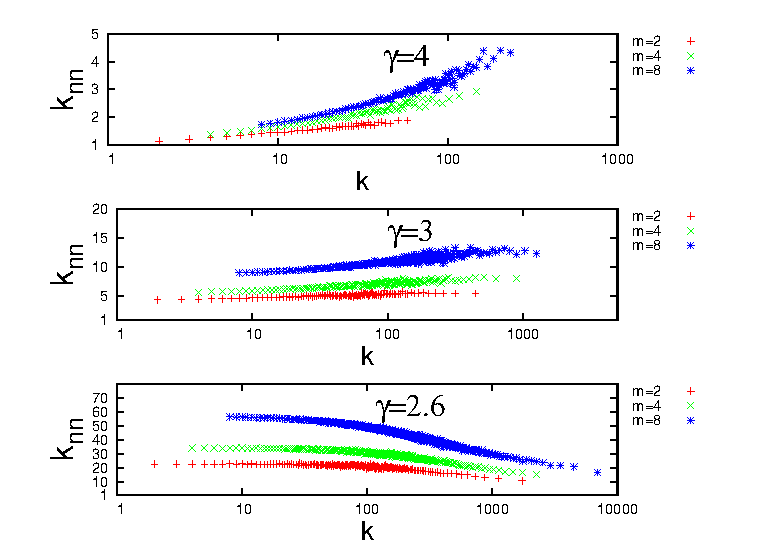
\includegraphics[scale=1.2]{./figures/correlation}
	\caption{Les corrélations des degrés dans le réseau aléatoire sans-échelle pour différentes valeurs de $m$ et de $\gamma$. Le nombre de nœuds est $n=10^4$ et le nombre de réalisations pour chaque simulations est $50$.}
	\label{correlation}
\end{figure}
\vspace{3cm}


\section{Les anciennes études sur les couches et le plus court chemin}
\subsection{Les couches}
\subsubsection{Contribution de Newman}
Newman \cite{Newman2010-456} a calculé l'expression des couches, c'est-à-dire le nombre moyen de nœuds, \nl, à distance $\ell$ depuis un nœud arbitraire pour un réseau aléatoire, son calcul est longue et un peu compliqué. On va essayer de résumer son calcul, soit $p_k^{(2)}$ est la probabilité qu'un nœud a exactement $k$ seconds voisins dans le réseau
\begin{equation}
p_k^{(2)}=\sum_{m=0}^{\infty}p_mP^{(2)}(k/m),
\end{equation}
avec $P^{(2)}(k/m)$ est la probabilité d'avoir $k$ seconds voisins étant donné que nous avons $m$ premiers voisins et $p_m$ est la distribution des degrés ordinaire.\\
La fonction génératrice de cette probabilité est 

\begin{align}
	g^{(2)}(z)&=\sum_{k=0}^{\infty}p_k^{(2)}z^{k}\nonumber\\
	&=\sum_{m=0}^{\infty}p_m\sum_{k=0}^{\infty}P^{(2)}(k/m)z^k\nonumber\\
	&=\sum_{m=0}^{\infty}p_m[g_1(z)]^m\nonumber\\
	&=g_0(g_1(z)).
	\label{p-generatrice-2}
\end{align}
Avec $g_0(z)=\sum_{k=0}^{\infty}p_kz^k$ et $g_1(z)=\frac{1}{g'_0(1)}\frac{dg_0}{dz}$.\\

Nous utilisons le même calcul pour calculer la distribution de probabilité du nombre de tiers voisins. Le nombre de tiers voisins est la somme des excès de chacun des seconds voisins. Ainsi, s'il y a $m$ seconds voisins, alors la distribution de probabilité $P^{(3)}(k/m)$ du nombre de tiers voisins a une fonction génératrice $[g_1(z)]m$ et la probabilité globale d'avoir $k$ troisième voisins est exactement analogue à l'équation
\begin{align}
g^{(3)}(z)&=\sum_{m=0}^{\infty}p_m^{(2)}\sum_{k=0}^{\infty}P^{(3)}(k/m)z^k\\
&=\sum_{m=0}^{\infty}p_m^{(2)}[g_1(z)]^m\nonumber\\
&=g^{(2)}(g_1(z))\nonumber\\
&=g_0(g_1(g_1(0))).
\end{align}
Par conséquence, la fonction génératrice du nombre de voisins à n'importe quelle distance $\ell$ peut être exprimée de cette façon
\begin{align}
g^{(\ell)}(z)&=\sum_{m=0}^{\infty}p_m^{(\ell-1)}\sum_{k=0}^{\infty}P^{(\ell)}(k/m)z^k\\
&=\sum_{m=0}^{\infty}p_m^{(\ell-1)}[g_1(z)]^m\nonumber\\
&=g^{(\ell-1)}(g_1(z)),
\label{p-generatrice-l}
\end{align}
avec $g^{(\ell)}(z)=g_0(...g_1(z)...)$, où dans $g_0$ il y a $\ell-1$ copie de $g_1$.\\
Il est généralement assez difficile d'extraire les expressions explicites des probabilités pour les nombres de seconds voisins dans le réseau.\\
Si nous supposons que notre distribution de degrés est une distribution de Poisson avec une moyenne $\km$, $p_k=\frac{\km^k}{k!}e^{-\km}$.\\
La moyenne d'une distribution est donnée par la dérivée première de sa fonction génératrice évaluée en $z=1$ et la dérivée de Eq.~\eqref{p-generatrice-2} est $\frac{dg^{(2)}}{dz}=g_0'(g_1(z))g_1'(z)$. En fixant $z=1$ et en rappelant que $g_1(1)=1$, on trouve que le nombre moyen $n_2$ des seconds voisins est
\begin{equation}
n_2=g_0'(1)g_1'(1),
\label{3-27}
\end{equation}
ainsi que $g_0'(1)=\km$ et $g_1'(1)=\frac{1}{\km}(\textless k^2\textgreater-\km)$, d'où on obtient
\begin{equation}
n_2=\textless k^2\textgreater-\km.
\end{equation}
Nous pouvons par utiliser le même principe de trouver le nombre moyen de voisins $n_{\ell}$ à n'importe quelle distance $\ell$. De Eq.~\eqref{p-generatrice-l} nous obtenons
\begin{equation}
\frac{dg^{(d)}}{dz}=g^{(d-1)'}(g_1(z))g_1'(z),
\end{equation}
sachant que nous avons $z=1$ nous pouvons écrire 
\begin{align}
n_{\ell}&=g^{(d-1)'}(1)g_1'(z)\\
&=n_{\ell-1}g_1'(1)\nonumber
\end{align}
de Eq.~\eqref{3-27} on a $g_1'(1)=\frac{n_2}{n_1}$, alors on obtient 
\begin{equation}
n_{\ell-1}=n_{\ell-1}\Big(\frac{n_2}{n_1}\Big),
\end{equation}

Nous pouvons alors écrire que la distribution des nœuds est sous la forme
\begin{equation}
 n_{\ell}=\Big(\frac{n_2}{n_1}\Big)^{\ell-1}n_1.
\end{equation} 

Cela signifie que \nl augmente ou diminue exponentiellement avec $\ell$ selon que $n_2$ est supérieur ou inférieur à $n_1$.

\subsubsection{Contribution de Cohen et al}
La construction de Cohen et al. \cite{Cohen-Havlinl2010-72,Kalisky-al2006} a basé sur le modèle de Bollobás \cite{Bollobas1985}. Le processus de construction tente d'exposer le réseau progressivement, en suivant une certaine méthode, ce qui permet de définir des couches  dans le graphe proposé. Nous définissons le nombre de nœuds dans le réseau, n, et nous associons les degrés avec les nœuds selon la loi de puissance $P(k)=Ck^{-\gamma}$, comme toujours $C=(\gamma-1)m^{\gamma-1}$ est la constante de normalisation avec $m$ est le degré minimal et $K=n^{\frac{1}{\gamma-1}}$ est le degré maximale.\\

A partir de ce que précède, chaque nœud du réseau dispose d'un nombre donné de liens sortants, nous appelons les liens ouverts, selon son degré choisi. Définissons $V$ comme l'ensemble des $n$ nœuds choisis, $c$ comme l'ensemble des liens sortant non connectés des nœuds de $V$, et $E$ comme l'ensemble des arêtes du graphe. En utilisant ces définitions, l'ensemble des liens dans $E$ est vide à ce stade, alors que l'ensemble des liens ouverts sortants dans $c$ contient tous les liens sortants non connectés dans le graphe. Dans la construction de Bollobás \cite{Bollobas1980}, les liens dans $c$ sont appariés de manière aléatoire, de sorte qu'à la fin du processus, $c$ est vide, et $E$ contient tous les liens correspondants.\\
Au lieu de cela,  nous partons du nœud de degré maximal, qui a le degré $K$, et le relions aléatoirement à $K$ liaisons ouvertes disponibles, supprimant ainsi ces liens ouverts de $c$. Nous avons maintenant exposé la première couche de nœuds, indexée comme $\ell=1$. Nous continuons maintenant à remplir la deuxième couche $\ell=2$ de manière similaire. Nous connectons tous les liens ouverts émergeant des nœuds de la couche $1$ vers des liens ouverts choisis au hasard. Ces liens ouverts peuvent être choisis parmi les nœuds de la même couche $1$ (créant ainsi une cycle) ou d'autres liens en $c$. Nous continuons jusqu'à ce que tous les liens ouverts émergeant de la couche $1$ soient connectés, remplissant ainsi la couche $\ell=2$. Généralement, pour former la couche $\ell+1$ à partir d'une couche arbitraire $\ell$, nous relions aléatoirement toutes les liaisons ouvertes émergeant de $\ell$ à d'autres liaisons ouvertes émergeant de $\ell$ ou choisies parmi les autres liaisons de $c$. Notez que lorsque nous avons formé la couche $\ell+1$, la couche $\ell$ n'a plus de liens ouverts. Le processus se poursuit jusqu'à ce que l'ensemble des liens ouverts, $c$, soit vide.\\
Le détaille de ce calcul est encore plus longue mais relativement aisé, En bref Cohen et al ont considéré un réseau sans échelle spécifique et ont étudié les couches entourant le nœud le plus connecté, ils ont obtenu une relation de récurrence pour \nl. Ces calculs semblent bien cadrer avec les données Internet réelles dans le cas particulier de $m=1$, où $m$ est le degré minimum dans le réseau. Deux régimes sont observés pour \nl: le premier est caractérisé par une croissance rapide, et le second descend de façon exponentielle.\\


Ces deux études ne sont pas satisfaisantes, car la première expression de Newman est une fonction monotone, c'est-à-dire soit croissante ou décroissante, ce qui est expérimentalement faux \cite{Cohen-Havlinl2010}, et dans le deuxième résultat, Cohen et al.  n'ont pas réussi à trouver une expression explicite, mais plutôt une suite de récurrences sans solution. En plus leurs expressions correspondent plus aux données d'Internet et ne représentent aucune généralité.
 
\subsection{Plus court chemin}
\label{PCC}
 Le plus court chemin (PCC) peut être le concept le plus intéressant dans les réseaux complexes et la théorie des graphes, principalement après la célèbre expérience de Milgram \cite{Mi1967}. Dans cette expérience, Milgram a clairement démontré le phénomène du petit monde dans les réseaux sociaux, ce qui signifie que deux personnes dans le monde sont en moyen séparées par des petites connexions intermédiaires.\\
 Nous pouvons citer les anciennes formules du PCC  en relation avec la valeur de l'exposant $\gamma$ comme ceci : Pour $2<\gamma<3$ on dit que le réseau est ultra-petit $\textless\ell\textgreater\sim \ln\ln(n)$ \cite{Cohen-Havlin2003,Do-al2003,Cohen-al2002,Chung-Lu2002,Fox-Bellwood2014,Hofstad-al2014}, pour $\gamma=3$ on dit que le réseau est petit-monde $\textless\ell\textgreater\sim\frac{\ln(n)}{\ln\ln(n)}$ \cite{Bollobas1985,Chung-Lu2002,Fronczak-al2004,Hofstad-al2004,Cohen-Havlin2009} et pour $\gamma>3$ le réseau est aussi petit-monde $\textless\ell\textgreater\sim\ln(n)$ \cite{Bollobas1985,Chung-Lu2002,Fronczak-al2004,Hofstad-al2004,Cohen-Havlin2009}.  

\section{Structure des couches dans les réseaux sans-échelle non corrélés}
        \subsection{L'étude théorique}
La couche dans un réseau complexe est définie comme l'ensemble des nœuds à la même distance d'un nœud arbitraire choisi. Dans un réseau sans-échelle, chaque nœud est lié à d'autres nœuds $k$ avec la probabilité $P(k)=Ck^{-\gamma}$, $k=m, m + 1, \ldots, K$. Où $C=(\gamma-1)m^{\gamma-1}$ est la constante de normalisation, $m$ et $K$ sont les seuils inférieur et supérieur de la distribution. $K=mn^{\frac{1}{\gamma-1}}$, avec $n$ est le nombre total de nœuds. \\
Nous construisons un réseau sans-échelle en choisissant aléatoirement un nœud de degré moyen $\km$, et dans chaque couche suivante, nous mettons le degré suivant le plus élevé jusqu'à que la couche soit pleine (Fig.~\ref{fig1}).\\
\begin{figure}[h]
	\centering
	\begin{tikzpicture}[scale=0.35]
	\tikzstyle{lien}=[-,thick,circle]
	\tikzset{individu/.style={draw,circle,scale=2,fill=black},individu/.default={green},scale=0.7}
	\node[individu,scale=0.3] (a0) at (-1,0) {};
	\node[individu,scale=0.6] (a1) at (2.5,-8) {};
	\node[individu,scale=0.52] (a2) at (-1,-9.18) {};
	\node[individu,scale=0.46] (a3) at (-4.5,-8) {};
	\node[individu,scale=0.44] (b1) at (5,-15.5) {};
	\node[individu,scale=0.42] (b2) at (3,-16.55) {};
	\node[individu,scale=0.4] (b3) at (1.,-17.25) {};
	\node[individu,scale=0.38] (b4) at (-1,-17.6) {};
	\node[individu,scale=0.36] (b5) at (-3.,-17.45) {};
	\node[individu,scale=0.34] (b6) at (-5,-16.92) {};
	\node[individu,scale=0.32] (b7) at (-7,-16.1) {};
	\node[individu,scale=0.3] (c1) at (8,-23.7) {};
	\node[individu,scale=0.28] (c2) at (5.2,-25.1) {};
	\node[individu,scale=0.26] (c3) at (3.,-25.9) {};
	\node[individu,scale=0.24] (c4) at (1,-26.28) {};
	\node[individu,scale=0.22] (c5) at (-1,-26.4) {};
	\node[individu,scale=0.2] (c6) at (-3,-26.3) {};
	\node[individu,scale=0.18] (c7) at (-5,-26.3) {};
	\node[individu,scale=0.16] (c8) at (-7,-26.1) {};
	\node[individu,scale=0.14] (c9) at (-9,-25.30) {};
	\node[individu,scale=0.12] (c10) at (-11,-24.10) {};
	\node[individu,scale=0.10] (c11) at (-13,-23.21) {};
	\draw[-,>=latex,dashed] (c11) to[bend right] (c1);
	\draw[-,>=latex,dashed] (b7) to[bend right] (b1);
	\draw[-,>=latex,dashed] (a3) to[bend right] (a1);
	\draw[lien] (a0) -- (a1);
	\draw[lien] (a0) -- (a2);
	\draw[lien] (a0) -- (a3);
	\draw[lien] (a1) -- (b1);
	%\draw[lien] (a1) -- (b2);
	%\draw[lien] (a1) -- (b3);
	\draw[lien] (a1) -- (b5);
	\draw[lien] (a1) -- (b4);
	\draw[lien] (a2) -- (b6);
	\draw[lien] (a2) -- (b2);
	%\draw[lien] (a2) -- (b6);
	\draw[lien] (a3) -- (b3);
	\draw[lien] (a3) -- (b7);
	\draw[lien] (b1) -- (c1);
	\draw[lien] (b1) -- (c2);
	%\draw[lien] (b1) -- (c4);
	\draw[lien] (b1) -- (c5);
	%\draw[lien] (b2) -- (c1);
	\draw[lien] (b2) -- (c4);
	\draw[lien] (b3) -- (c3);
	\draw[lien] (b4) -- (c7);
	\draw[lien] (b3) -- (c8);
	\draw[lien] (b2) -- (c6);
	\draw[lien] (b5) -- (c10);
	\draw[lien] (b6) -- (c9);
	%\draw[lien] (b7) -- (c7);
	\draw[lien] (b7) -- (c11);
	\draw (-16.5,-7.5) node[right]{$l_1$,$n_1=\textless k \textgreater$};
	\draw (-13,-15.7) node[right]{$l_2$,$n_2$};
	\draw (-19.,-23) node[right]{$l_3$,$n_3$};
	\draw (3.3,-8) node[right]{$K_1=K$};
	\draw (5.4,-15.5) node[right]{$K_2$};
	\draw (8.1,-23.7) node[right]{$K_3$};
	\end{tikzpicture}
	\caption{Illustration du réseau construit. La taille des cercles pleins (nœuds) est le degré dépendant. Le degré maximum de couche $\ell$ est $K_{\ell}$.\\}
	\label{fig1}
\end{figure}

Évidemment, la première couche contiendra les premiers voisins $\km$ du nœud de départ, alors $n_1=\km$. Cela ne représente pas un réseau particulier, mais c'est juste une description idéalisée de tout réseau sans échelle. \\
Pour les grands réseaux non corrélés, la structure arborescente peut être supposée et les cycles dans la même couche sont négligés \cite{Cohen-Havlin2003,Cohen-Havlin2009}. Par la suite, la probabilité $ p_{\ell} $ qu'un nœud de la couche $n_\ell$ soit lié à un autre nœud n'appartenant pas aux premiers $\ell$ couches est $p_{\ell}=\frac{\kappa_{\ell}-1}{n}$, où $\kappa_{\ell}$ est le degré moyen des nœuds appartenant à la couche $n_\ell$ et le $-1$ est dû au lien de la couche précédente. \\
La probabilité que des nœuds parmi $n-n_1-1$ ne soient lié à aucun nœud dans $\ell=1$ est $(1-p_1)^{n_1}$, alors la probabilité que ces nœuds soient liés aux nœuds dans $\ell=1$ est $1-(1-p_1)^{n_1}$. Le nombre de nœuds dans $\ell=2$ est alors donné par $n_2=(1- (1-p_1)^{n_1})(n-n_1-1)$. La généralisation pour \nl est simple, on obtient:
\begin{align}
n_{\ell}= (1-(1-p_{\ell-1})^{n_{\ell-1}})(n-\sum_{j=1}^{\ell-1} n_j-1),
\label{eq1}
\end{align}
lorsque $n$ est grand $p_{\ell}\ll1 \Longrightarrow (1-p_{\ell-1})^{n_{\ell-1}}\simeq e^{-p_{\ell-1}n_{\ell-1}} $. Eq.~\eqref{eq1}
peut être facilement manipulé pour obtenir:
\begin{align}
n_{\ell} &=
\begin{cases}
\km & \text{si}\qquad \ell=1 \\
(n-1-n_1)(e^{-\sum_{j=1}^{\ell-2}p_j n_j}-e^{-\sum_{j=1}^{\ell-1}p_j n_j}) & \text{si}\qquad \ell \ge 2.
\end{cases}
\label{eq2}
\end{align}
L'équation ci-dessus peut être simplifiée en développant les sommes en exponentielles. $p_{\ell}$ est $\kappa_{\ell}$-dépendante, qui dépend à son tour de $\gamma$ et du degré maximal dans la couche $\ell$, $K_{\ell}$. D'abord on donne l'expression de $\kappa_{\ell}$ quand $K_{\ell}\gg m$, et ensuite on développe la somme sur $n_j$.
\begin{align}
\kappa_{\ell} =\frac{<k_{\ell}^2>}{\textless k_{\ell} \textgreater}=&
\begin{cases}
\Big(\frac{\gamma-2}{\gamma-3}\Big)m & \text{si} \qquad \gamma >3 \\ 
m (\log(K_{\ell})-\log(m))  & \text{si} \qquad \gamma =3 \\
\Big(\frac{\gamma-2}{3-\gamma}\Big)m^{\gamma-2} K_{\ell}^{3-\gamma}  & \text{si} \qquad 2<\gamma<3 \\
\frac{K_{\ell}-m}{\log(K_{\ell})-\log(m)} & \text{si} \qquad \gamma=2.
\end{cases}
\label{eq4}
\end{align}
Lorsque $\gamma=2$, le degré maximum $K_1$ est de l'ordre du nombre total de nœuds, c'est-à-dire que presque tous les nœuds sont connectés au nœud de degré maximal. Le réseau peut contenir un maximum de deux couches, avec $n_1=\km$ et $n_2=n-\km $. \\
Quand $2\textless \gamma \textless 3$, le réseau est encore très hétérogène. $\kappa_{\ell} $ est couche-dépendent, il dépend du degré maximal $K_{\ell} $ de la couche $\ell$ (Eq.~\eqref{eq4}). L'étape suivante de nos calculs consiste à relier $\kappa_{\ell}$ à $\kappa_1$. Le nombre de nœuds entre le premier et le $(\ell-1)^{\text{ème}}$ couches est donné par:
\begin{align}
\sum_{j=1}^{\ell-1}n_j&=n\int_{K_{\ell}}^{K_1} P(k)dk \nonumber \\
&=nm^{\gamma-1}(K_{\ell}^{1-\gamma}-K_1^{1-\gamma})\simeq nm^{\gamma-1} K_{\ell}^{1-\gamma},
\label{eq5}
\end{align}
où nous avons utilisé $K_1\gg K_{\ell}$ pour $n$ assez grand. Dans ce cas où $2\textless \gamma \textless 3$, $\kappa_{\ell}\gg 1$, alors
\begin{align}
\sum_{j=1}^{\ell-1}n_j&=\km+\km(\kappa_1-1)+\km(\kappa_1-1)(\kappa_2-1)+\ldots+\km(\kappa_1-1)(\kappa_2-1)\ldots(\kappa_{\ell-1}-2)\nonumber \\
&\approx\km\kappa_1\kappa_2\ldots\kappa_{\ell-2},
\label{eq6}
\end{align}
on en déduit
$K_{\ell}=\Big(\frac{\km\kappa_1\kappa_2\ldots\kappa_{\ell-2}}{nm^{\gamma-1}}\Big)^{\frac{1}{1-\gamma}}$.\\
Le degré moyen des voisins à distance $\ell $ peut maintenant être exprimé comme ceci :
$\kappa_{\ell}=\frac{\gamma-2}{3-\gamma}m\Big(\frac{n}{\km\kappa_1\kappa_2\ldots\kappa_{\ell-2}}\Big)^{\frac{3-\gamma}{\gamma-1}}$, ce qui conduit à la relation de récurrence $\kappa_{\ell}=\kappa_{\ell-1}
\Big(\kappa_{\ell-2}\Big)^{\frac{\gamma-3}{\gamma-1}}$.  Quand $\gamma$ est dans $]2,3[$ nous avons généralement
$\kappa_{\ell-2} \gg \kappa_{\ell-1}$  mais depuis $\mid\frac{\gamma-3}{\gamma-1}\mid<1$, on considère que $\Big(\kappa_{\ell-2}\Big)^{\frac{\gamma-3}{\gamma-1}}\approx
\Big(\kappa_{\ell-1}\Big)^{\frac{\gamma-3}{\gamma-1}}$. Enfin, on obtient $\kappa_{\ell}=\kappa_1^{\Big(\frac{2\gamma-4}{\gamma-1}\Big)^{\ell-1}}$.\\
Nous sommes maintenant prêts de calculer la somme dans l'Eq.~\eqref{eq2}:
\begin{align}
\sum_{j=1}^{l} p_jn_j&=\sum_{j=1}^{l}\frac{\kappa_j}{n}\Big(\km\kappa_1\kappa_2\ldots\kappa_{j-1}\Big) \nonumber\\ 
&\approx \frac{\kappa_{\ell}}{n}\Big(\km\kappa_1\kappa_2\ldots\kappa_{\ell-1}\Big) \nonumber \\
&\approx \frac{\km}{n}\kappa_1^{1+\beta+\beta^2+\ldots+\beta^{\ell-1}} \nonumber \\
&\approx \frac{\km}{n}\kappa_1^{\frac{1-\beta^{\ell}}{1-\beta}},
\label{eq7}
\end{align}
où $\beta=\frac{2\gamma-4}{\gamma-1}$. En prenant $n-n_1-1 \approx n$, Eq.~\eqref{eq2} peut être écrit pour $2\textless \gamma \textless 3$ comme:
\begin{align}
n_{\ell} &=
\begin{cases}
\km & \text{if}\qquad \ell=1 \\
n\Big(e^{-\frac{\km}{n}\kappa_1^{\frac{1-\beta^{\ell-2}}{1-\beta}}}-e^{-\frac{\km}{n}\kappa_1^{\frac{1-\beta^{\ell-1}}{1-\beta}}}\Big) & \text{if}\qquad \ell \ge 2.
\end{cases}
\label{eq8}
\end{align}
Quand $\gamma> 3 $, les hubs ne sont pas grands, et les propriétés caractéristiques du réseau sont similaires à celles des réseaux aléatoires ER.
 $\kappa_{\ell}$ est couche-indépendant comme indiqué dans Eq.~\eqref{eq4}.
Alors $\sum_{j=1}^{\ell-1}p_j n_j=\frac{\kappa'}{n}\sum_{j=1}^{\ell-1}n_j$, où $\kappa'=\kappa-1$.  
\begin{align}
\sum_{j=1}^{\ell}n_j &=\km+\km(\kappa_1-1)+\km(\kappa_1-1)(\kappa_2-1)+\ldots+\km(\kappa_1-1)(\kappa_2-1)\ldots(\kappa_{\ell-1}-1) \nonumber\\
&=\km+\km\kappa'+\km\kappa'^2+\ldots+\km\kappa'^{\ell-1}=\km\frac{1-\kappa'^{\ell}}{1-\kappa'}. 
\label{eq9}
\end{align}
Eq.~\eqref{eq2} peut être écrit pour $\gamma>3$ comme:
\begin{align}
n_{\ell} &=
\begin{cases}
\textless k \textgreater & \text{if}\qquad \ell=1 \\
n(e^{-\frac{\textless k \textgreater}{n}\kappa'\frac{1-\kappa'^{\ell-2}}{1-\kappa'}}-e^{-\frac{\km}{n}\kappa'\frac{1-\kappa'^{\ell-1}}{1-\kappa'}}) & \text{if}\qquad \ell \ge 2.
\end{cases}
\label{eq10}
\end{align}
\begin{figure}[h!]
	\centering
	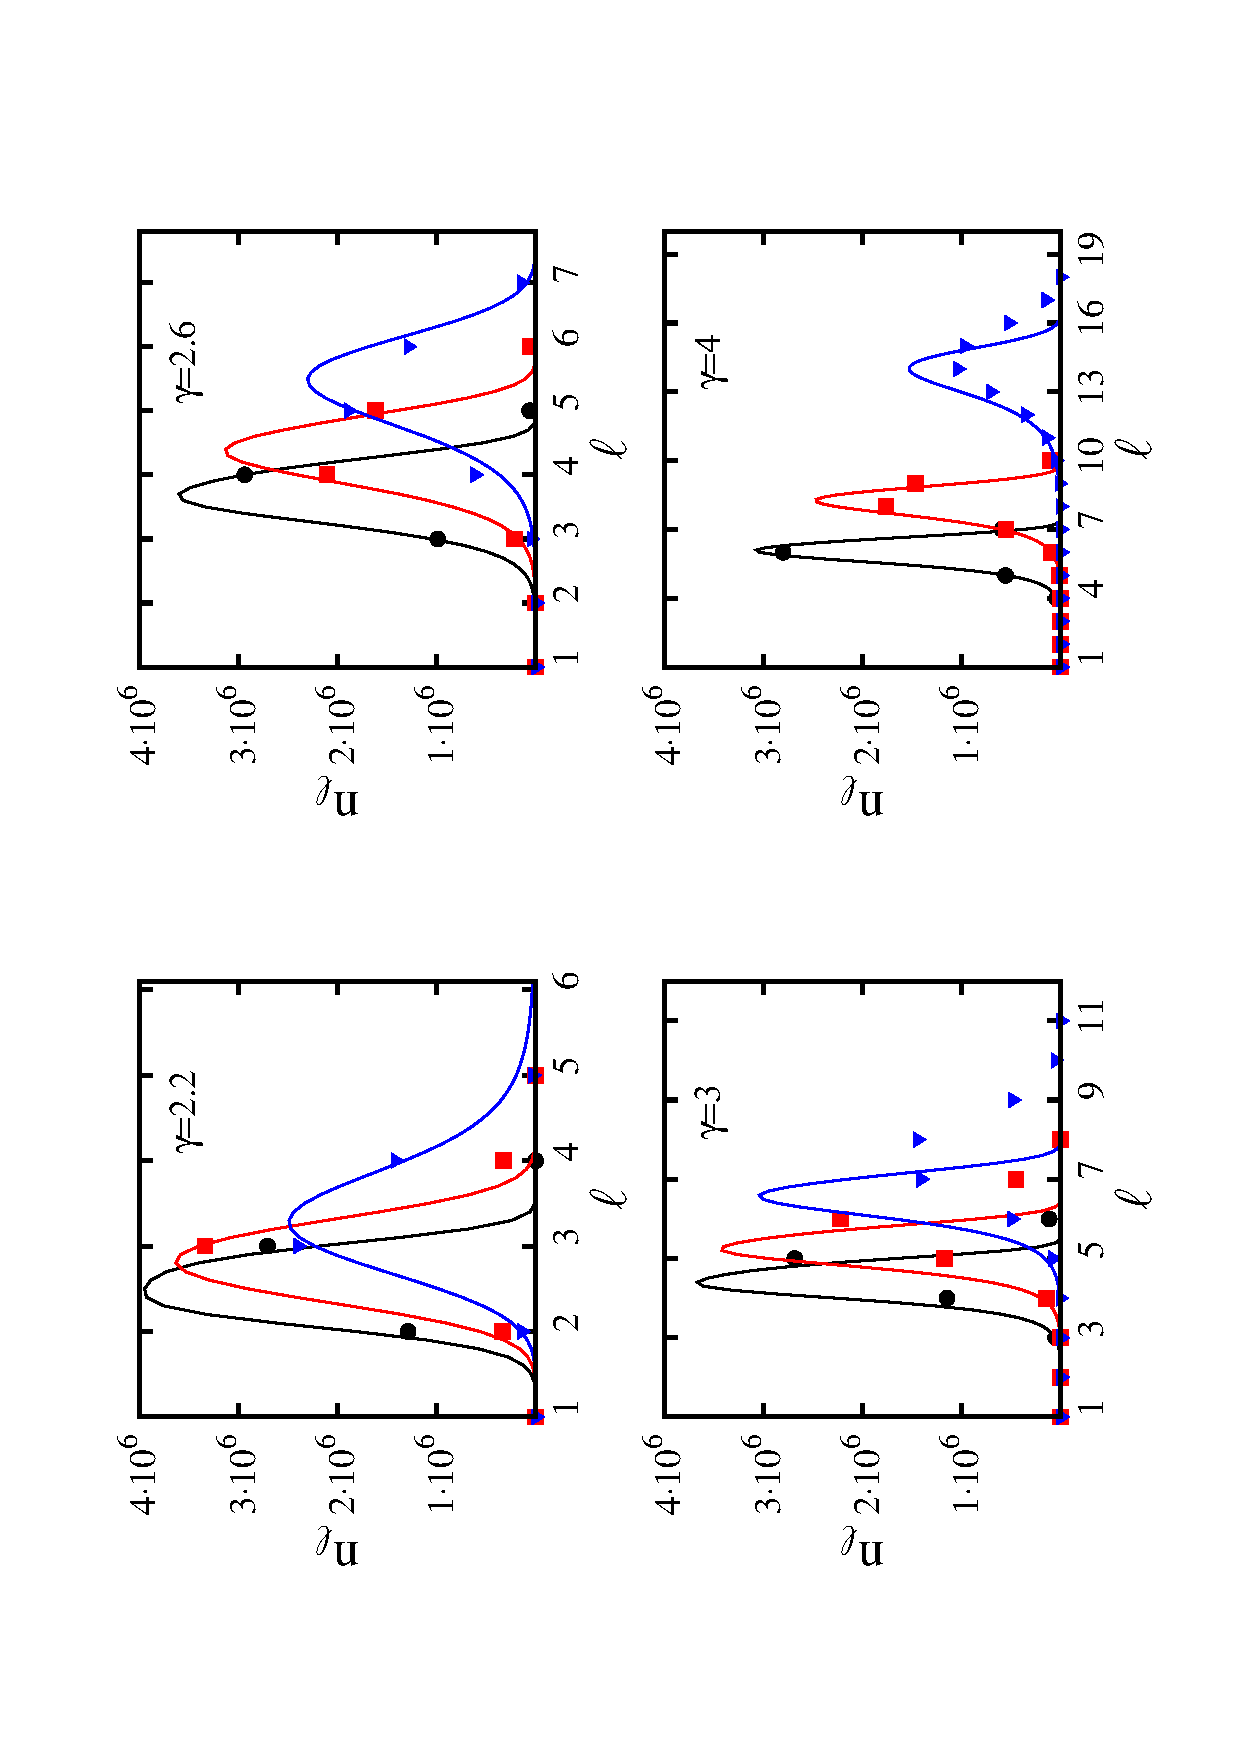
\includegraphics[angle=-90,scale=0.65]{./figures/fig2-3}
	\caption{Nombre de nœuds dans chaque couche pour différentes valeurs de $ \gamma $. Les lignes pleines sont Eq.~\eqref {eq8} et Eq.~\eqref{eq10}. Les symboles sont des simulations d'un réseau de taille $n=4\times10^6$ et une moyenne de $200$ réalisation pour chaque point. Les couleurs noir, rouge et bleu se réfèrent respectivement à $ m = 8, 4 $ et $ 2 $.}
	\label{fig2-3}
\end{figure}

Le cas $\gamma=3$ est le plus problématique. C'est le point où la structure du réseau change radicalement, nous constatons la présence de multiples grands hubs et un second moment  $\textless k^2 \textgreater$ diverge pour $\gamma<3$, par contre nous remarquons une absence des hubs importants et un $\textless k^2  \textgreater$ fini pour $\gamma>3$.
Dans notre approche, le problème se pose lors du calcul de $\sum_{j=1}^{l}p_jn_j$. Néanmoins, à ce point de transition ($\gamma=3$), certaines propriétés du réseau se comportent presque comme celles correspondant à $\gamma>3$.
Principalement, le PCC est mise à l'échelle avec $n$ comme $\frac {\log(n)}{\log(\log(n))}$ \cite{Bollobas-Riordan2004}, et $\textless k^2  \textgreater$ reste fini. Ensuite, nous utilisons Eq.~\eqref{eq10} pour calculer \nl dans ce cas. \\
Dans la Fig.~\ref{fig2-3}, nous représentons \nl en fonction de $\ell$ pour différentes valeurs de $\gamma$ et $m$, en général, un excellent accord entre la théorie et les simulations est observé. Pour $\gamma=3$, l'accord est moins bon, principalement due au fait que le réseau est encore hétérogène et que les hubs sont toujours présents, alors que nous avons supposé l'homogénéité du réseau pour calculer $\sum_{j=1}^{l} p_jn_j$ (Eq.~\eqref{eq9}). Nous observons aussi peu de différences en \nl entre la théorie et les simulations lorsque $ \gamma = 4 $ et $ m = 2 $. Ceci est causé par une augmentation relative de la proportion de cycles dans les mêmes couches. Ainsi, la structure arborescente parfaite, qui est l'hypothèse principale dans le calcul de \nl, n'est plus vraie. La Fig.~\ref{fig3-3} montre clairement l'augmentation relative des cycles quand $ m $ est abaissé, et $ \gamma $ augmenté.\\
Nos résultats analytiques pour \nl sont également comparés aux réseaux du monde réel. Nous observons à partir de Fig.~\ref{fig2-3} que \nl augmente et diminue de différentes manières. Les manipulations de Eq.~\eqref{eq8} et Eq.~\eqref {eq10} sont nécessaires pour extraire une information détaillée sur les queues de la distribution des nœuds. \\ Pour $n$ grand, Eq.~\eqref{eq8} pour $\ell>1$ peut être approché comme:
\begin{align}
n_{\ell}&=n\Big(e^{-\frac{\km}{n}\kappa_1^{\frac{1-\beta^{\ell-2}}{1-\beta}}}-e^{-\frac{\km}{n}\kappa_1^{\frac{1-\beta^{\ell-1}}{1-\beta}}}\Big) \nonumber \\
&\approx -n \frac{\partial \Big(e^{-\frac{\km}{n}\kappa_1^{\frac{1-\beta^{\ell-\frac{3}{2}}}{1-\beta}}} \Big) }{\partial \ell} \nonumber \\
&\approx -\frac {\km \log(\kappa_1) \log(\beta)} {1-\beta} \beta^{\ell-\frac{3}{2}} \kappa_1^{\frac{1-\beta^{\ell-\frac{3}{2}}}{1-\beta}}e^{-\frac{\km}{n}\kappa_1^{\frac{1-\beta^{\ell-\frac{3}{2}}}{1-\beta}}}, 
\label{eq11}
\end{align}
où $ \ell-\frac{3}{2} $ est utilisé à la place de $ \ell-1$ pour améliorer la différenciation avec la règle du point central. Quand $\kappa_1^{\frac{1-\beta^{\ell-\frac{3}{2}}}{1-\beta}}\ll\frac{n}{\km}$,  $e^{-\frac{\km}{n}\kappa_1^{\frac{1-\beta^{\ell-\frac{3}{2}}}{1-\beta}}}\approx 1$, le terme dominant dans l'équation Eq.~\eqref{eq11} est $\kappa_1^{\frac{1-\beta^{\ell-\frac{3}{2}}}{1-\beta}}$, celle-ci peut écrire comme
\begin{align}
\kappa_1^{\frac{1-\beta^{\ell-\frac{3}{2}}}{1-\beta}}&=e^{\ln(\kappa_1^{\frac{1-\beta^{\ell-\frac{3}{2}}}{1-\beta}})}\nonumber\\
&= e^{\frac{1-\beta^{\ell-\frac{3}{2}}}{1-\beta}\ln(\kappa_1)},
\end{align}
il est difficile d'extraire la loi exacte de \nl à partir de l'expression au-dessus, mais de façon générale on peut dire que \nl dans le premier régime, $\kappa_1^{\frac{1-\beta^{\ell-\frac{3}{2}}}{1-\beta}}\ll\frac{n}{\km}$, augment rapidement comme un double exponentielle, et après avoir atteint son maximum à $\kappa_1^{\frac{1-\beta^{\ell-\frac{3}{2}}}{1-\beta}}=\frac{n}{\km}$, \nl diminue comme un triple exponentiel
$e^{-\frac{\km}{n}\kappa_1^{\frac{1-\beta^{\ell-\frac{3}{2}}}{1-\beta}}}$ quand $\kappa_1^{\frac{1-\beta^{\ell-\frac{3}{2}}}{1-\beta}}\gg\frac{n}{\km}$ (deuxième régime).\\
Les résultats obtenus semblent étonnants, mais le fait que dans le cas où $2<\gamma<3$ le réseau est définit comme ultra-petit monde, c'est-à-dire $\ell\sim \ln\ln(n)$, explique qu'il est normale que \nl augmenter comme un double exponentiel.
\begin{figure}[h]
	\begin{center}
		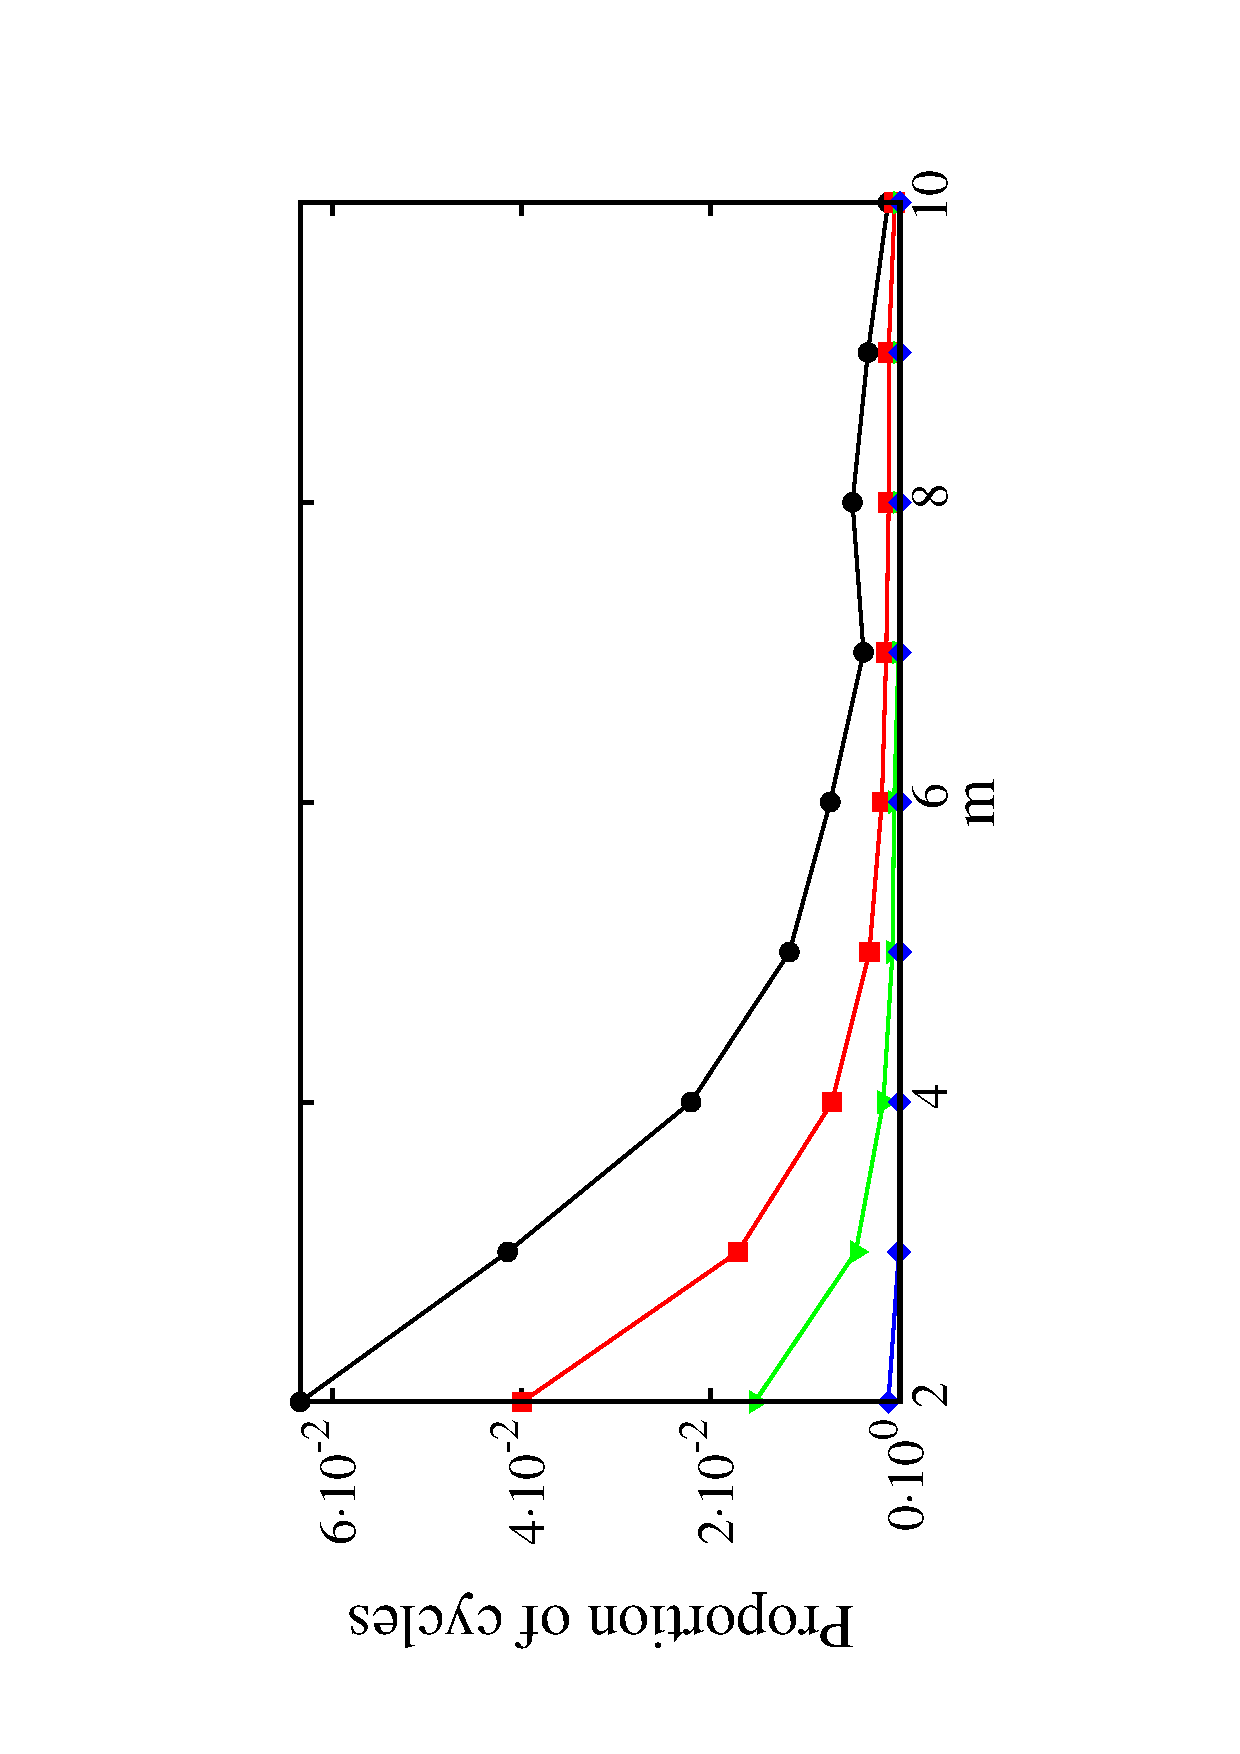
\includegraphics[angle=-90,scale=0.5]{./figures/fig3-3}
	\end{center}
	%\vspace{-10mm}
	\caption{Proportion de cycles dans les couches par rapport à $ m $. De haut en bas, $ \gamma $ est respectivement $ 4, 3, 2.6 $ et $ 2.2 $. Nombre de nœuds $ n = 4.10^6 $, le nombre de points pour chaque simulation est $200 $.}
	\label{fig3-3}
\end{figure}

De la même manière, Eq.~\eqref{eq10} peut être écrire comme
\begin{align}
n_{\ell}&= n(e^{-\frac{\textless k \textgreater}{n}\kappa'\frac{1-\kappa'^{\ell-2}}{1-\kappa'}}-e^{-\frac{\km}{n}\kappa'\frac{1-\kappa'^{\ell-1}}{1-\kappa'}})\nonumber\\
&\approx n\big(e^{-\frac{\km}{n}\kappa'^{\ell-2}}-e^{-\frac{\km}{n}\kappa'^{\ell-1}}\big)\nonumber\\
&\approx n\frac{\partial e^{-\frac{\km}{n}\kappa'^{\ell-\frac{3}{2}}}}{\partial \ell}\nonumber\\
&\approx\km\ln(\kappa')\kappa'^{\ell-\frac{3}{2}}e^{-\frac{\km}{n}\kappa'^{\ell-\frac{3}{2}}},
\end{align}
nous déduisons alors qu'on a une croissance de loi exponentiel pour $\kappa'^{\ell-\frac{3}{2}} \ll \frac{n}{\km}$ , et une décroissance de double exponentielle pour $\kappa'^{\ell-\frac{3}{2}} \gg \frac{n}{\km}$, car $\kappa'^{\ell-\frac{3}{2}}=e^{(\ell-\frac{3}{2})\ln(\kappa')}$. La même remarque  concernant la croissance exponentiel des couches, le fait que dans ce cas où $\gamma\geq3$ le réseau est définit comme petit-monde, c'est-à-dire $\ell\sim\ln(n)$, cela montre que la croissance exponentiel est normale. 
%\begin{figure}[h!]
%	\centering
%\includegraphics[scale=0.5,angle=-90]{./figures/%fig-queue2}
%	\caption{Comparaison entre la loi %exponentielle (ligne pointillé) et les queues de %quelque réseaux réels:\\
%	 Rovira (diamant): C'est le réseau de %communication par e-mail de l'Université Rovira %i Virgili de Tarragone, dans le sud de la %Catalogne, en Espagne. Les nœuds sont des %utilisateurs et chaque bord représente qu'au %moins un e-mail a été envoyé, la taille de %réseau $n=5451$ et $\gamma=6.771$.\\
	% baidu-internal-link (triangle): C'est le %réseau dirigé d'hyperliens entre les %articles de l'encyclopédie en ligne chinoise %Baidu, sa taille $n=17794839$ et $\gamma=2.291$\\ Twitter-ICWCM (carre):  \\
%Digg (étoile): C'est le réseau de réponse du %site d'informations sociales Digg. Chaque nœud %du réseau est un utilisateur du site Web, et %chaque arête dirigée indique qu'un utilisateur a %répondu à un autre utilisateur, sa taille est %$n=30398$ et $\gamma=2.691$.  Tous les résultats %empiriques ont été extraites du sites %"http://konect.uni-koblenz.de/networks/"}
%	\label{queues}
%\end{figure}
En outre, la décroissance par un triple exponentiel pour $2<\gamma<3$ et double exponentiel pour $\gamma\geqslant3$ est surprenant. Néanmoins il doit savoir que ces comportements sont apparaissent au loin de la couche maximale, ainsi que les comparaisons avec les simulations numériques Fig.~\ref{fig2-3}  et les données réelles Fig.~\ref{couch-reel} confirment nos résultats obtenus.
% ainsi que la décroissance dans des couches %dans quelque réseaux réels montre des chutes %très rapide que l'exponentiel (voir %Fig.~\ref{queues}), 

\subsection{Comparaison avec les données réels}
La Fig.~\ref{couch-reel} représente une comparaison entre nos équations et le réseau Hollywoodien de $2283910$ acteurs. En général nos équations sont très en accord avec ce réseau réel, ce qui donne une importance supplémentaire à notre travail concernant ce problème de couches dans les réseaux sans-échelle. 
\begin{figure}[h!]
	\centering
	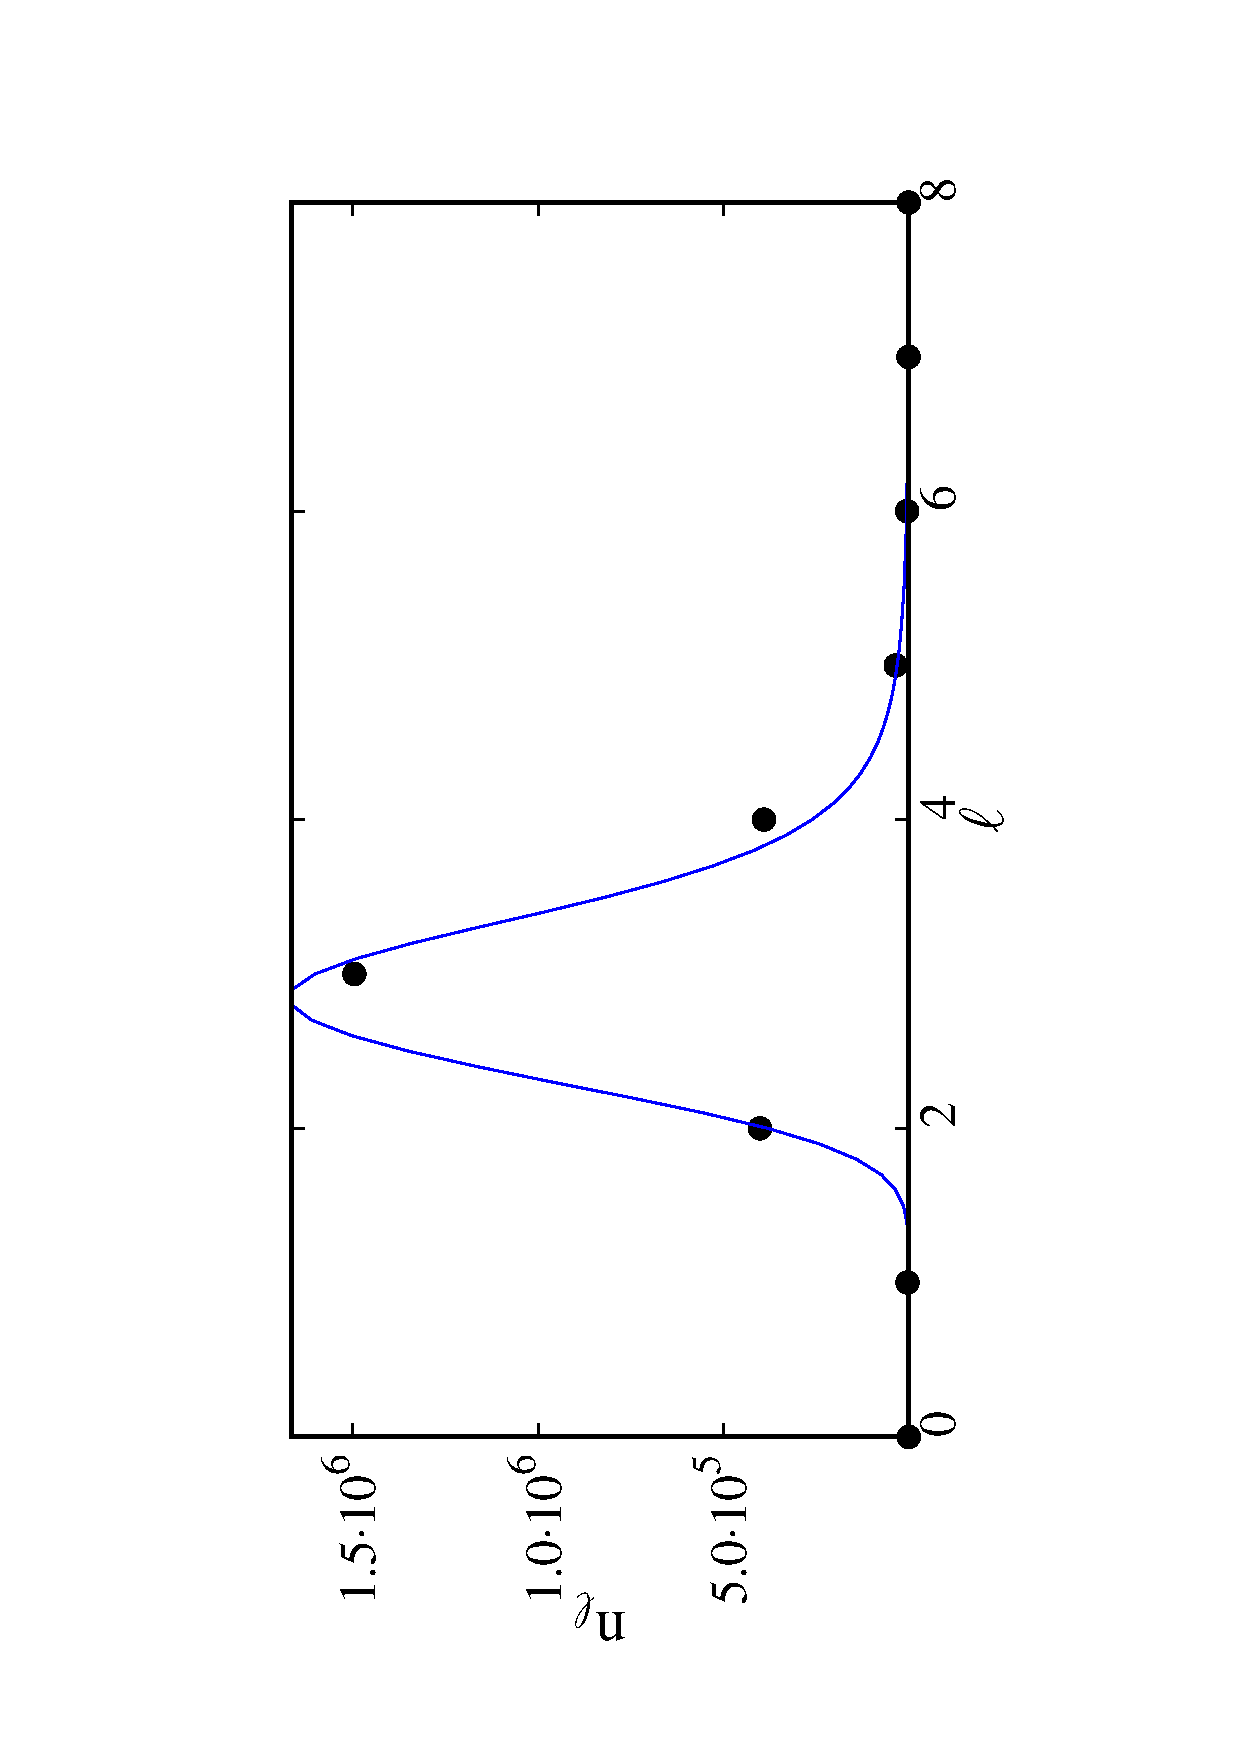
\includegraphics[scale=0.4,angle=-90]{./figures/couch-reel2}
	\caption{Comparaison entre les données empiriques (cercle) et notre équation théorique (ligne continue): Les cercles représentent les couches du réseau d’acteurs Hollywoodien de $2283910$ acteurs et de $\gamma=2.13$ lorsque Kevin Bacon est au centre du réseau et la ligne continue représente l'Eq.~\eqref{eq8} avec les mêmes valeurs $\gamma$ et $n$ du réseau Hollywoodien. Les résultats empiriques ont été extraits du site: "http://oracleofbacon.org/center.php".}	
	\label{couch-reel}
\end{figure}
    
\section{Plus court chemin dans les réseaux sans-échelle non corrélés }
   \subsection{L'étude théorique}
   \label{pcc}
   Nous déduisons le PCC dans les réseaux sans-échelle non corrélés à partir de la distribution des nœuds, \nl. En fait, la forme quasi-symétrique de \nl dans la Fig.~\ref{fig2-3} suggère que le PCC correspond à la distance à laquelle \nl est maximal. \\ Nous commençons par le cas le plus simple $\gamma=2$. Comme déjà mentionné, il y a un maximum de deux couches dans le réseau, le PCC peut être écrit comme:
   \begin{align}
   	\textless \ell \textgreater=\frac{\km+2(n-\km)}{n},
   	\label{eq14}  
   \end{align}
qui tend vers $2$ pour un grand $n$. Cela signifie que presque tous les nœuds sont connectés en moyen au nœud de degré maximal. \\
Quand $ 2<\gamma<3 $, aucune solution pour $\frac{\partial n_{\ell}}{\partial\ell}=0$ ne peut être trouvée directement à partir de l'Eq.~\eqref{eq8}, à la place nous utilisons l'approximation donnée dans Eq.~\eqref{eq11}, où \ nl est maximal quand $\kappa_1^{\frac{1-\beta^{\textless \ell \textgreater-\frac{3}{2}}}{1-\beta}}=\frac{n}{\km}$. Après avoir remplacé $\kappa_1 $ et $K_1$ par leurs expressions correspondantes, on obtient:
\begin{align}
	\textless \ell \textgreater=\frac{\log\big(1-\frac{\log(n)-\log(\km)}{\log(n)+\frac{\gamma-1}{3-\gamma}\log(\frac{\gamma-2}{3-\gamma}m)}\big)}{\log\big(\frac{2\gamma-4}{\gamma-1}\big)}+\frac{3}{2}.
	\label{eq12}
\end{align}
pour $n$ grand, $\textless \ell \textgreater \approx -\frac{\log(\log(n))}{\log(\beta)}$.
Cette forme d'échelle est derrière la nomenclature mondiale ultra-petite \cite{Cohen-Havlin2003}, et est largement acceptée pour cette gamme de $\gamma $ \cite{Do-al2003,Cohen-al2002,Chung-Lu2002,Fox-Bellwood2014,Hofstad-al2014}.\\
Pour $\gamma\ge 3 $, le PCC peut être déduit de Eq.~\eqref{eq10} en résolvant $\frac{\partial n_{\ell}}{\partial\ell}=0$. Cela donne:
\begin{align}
	\textless \ell \textgreater=\frac{\log (n)}{\log(\kappa')}+\frac{\log(\log(\kappa'))-\log(\km)}{\log(\kappa')}+1.
	\label{eq13}
\end{align}
Si $\gamma>3$, $\kappa$ est constant (Eq.~\eqref{eq4}). Pour un grand $n$, $\textless\ell\textgreater\approx\frac{\log(n)} {\log (\kappa')}$, qui est la forme d'échelle rapportée dans de nombreux autres travaux \cite{Bollobas1985,Chung-Lu2002,Fronczak-al2004,Hofstad-al2004,Cohen-Havlin2009}, et connu comme le comportement du petit monde. \\
Quand $\gamma=3$, $\kappa$ dépend de $K$, qui dépend à son tour de $n$. Prenant $\kappa=m(\log(K)-\log(m))$ et $K=mn^{\frac{1}{\gamma-1}}$, nous trouvons pour  $n$ grand, $\textless\ell\textgreater\approx \frac{\log(n)} {\log(\log(n))} $. Ce résultat est en accord avec les travaux précédents \cite {Chung-Lu2002,Cohen-Havlin2003,Fronczak-al2004,Bollobas-Riodan2002}, et confirme le cas particulier de $ \gamma = 3 $. En effet, la présence des hubs rend les distances entre les nœuds plus petites que celles où les hubs sont absents ($\gamma>3$), en même temps les hubs ne sont pas suffisamment grands pour faire des distances ultra-petites comme $2<\gamma<3$.  
 
Comme nous avons signalé dans la Section.~\ref{PCC}, les travaux importants \cite{Do-al2003,Cohen-Havlin2003} dans ce sujet donnent seulement l'allure du PCC pour les grandes valeurs de $n$. L'exception est la contribution de Fronczak et  al. \cite{Fronczak-al2004} où ils ont trouvé les expressions du PCC basées sur les paramètres du réseau, leurs équations ont prédit que le PCC tend vers une valeur constante lorsque $n$ tend vers l'infini pour $2<\gamma<3$, mais cela n’est pas vrai selon les simulations numériques (voir Fig.~\ref{fig4-3}) et tous les autres résultats existant dans la littérature \cite{Do-al2003,Cohen-al2002,Chung-Lu2002,Fox-Bellwood2014,Hofstad-al2014,Cohen-Havlin2003}. De la même figure (Fig.~\ref{fig4-3}) on voit que nos résultats sont parfaitement en accord avec les simulations pour $\gamma\neq3$, pour $\gamma=3$ nos résultat sont très proches et possèdent la même allure que les simulations, ils sont également très similaires au ceux de \cite{Fronczak-al2004}.
 \begin{figure}[h]
 	\centering
 	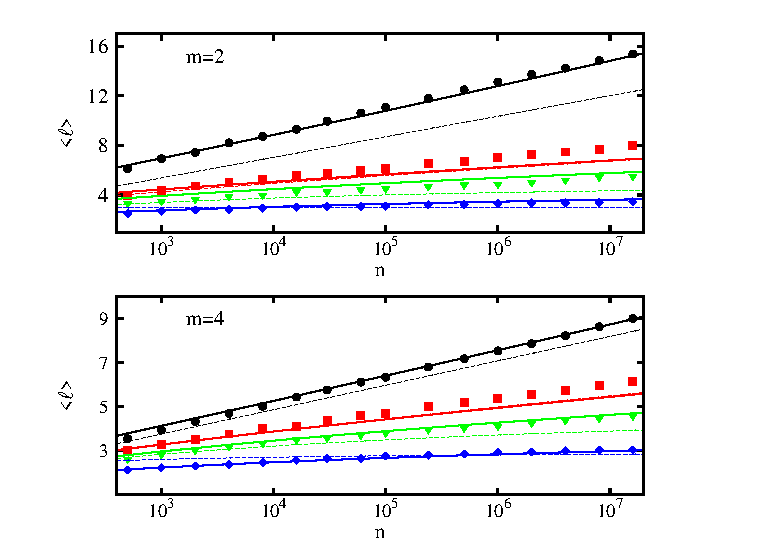
\includegraphics[scale=1.45]{./figures/fig4-3}
 	\caption{La longueur moyenne du trajet en fonction du nombre de nœuds. Les valeurs de $\gamma$ de haut en bas sont respectivement $ 4, 3, 2.6 $ et $ 2.2 $. Les lignes pleines correspondent à l'équation Eq.~\eqref{eq12} et à l'équation Eq.~\eqref{eq13}. Chaque simulation est moyennée à plus de $200 $.}
 	\label{fig4-3}
 \end{figure}
 
\section{conclusion} 
Dans ce chapitre, nous avons étudié en détail certains aspects fondamentaux des réseaux sans-échelle non corrélés. Avec des étapes et des hypothèses simples, nous avons obtenu des expressions explicites, en fonction de l'exposant de degré $\gamma$, pour le nombre des nœuds à une distance donnée d'un nœud arbitraire, \nl\nolinebreak, ainsi qu'une description précise de la formule de distribution \nolinebreak.
Profitant de la formule de distribution \nl, nous avons pu déduire l'expression explicite du PCC. Les expressions obtenues reproduisent les formes de mise à l'échelle connues pour différentes plages de $\gamma$. Autrement dit, le monde ultra-petit pour $2<\gamma<3$, et le petit monde pour $\gamma\ge 3$. Nos résultats théoriques concordent très bien avec les simulations, sauf dans le cas de $\gamma=3$, où nous avons observé la même forme, comme pour les autres valeurs de $\gamma$, dans les queues de \nl, mais avec une notable différence dans la position du maximum. Cette différence n'affecte pas la forme de mise à l'échelle du PCC pour cette valeur de $\gamma$.